\chapter{Конструкторский раздел}
\label{cha:design}

\section{Модель}
IDEF0 модель задачи вычисления редакционного расстояния приведена на рисунке 2.1.
\begin{figure}
    \centering
    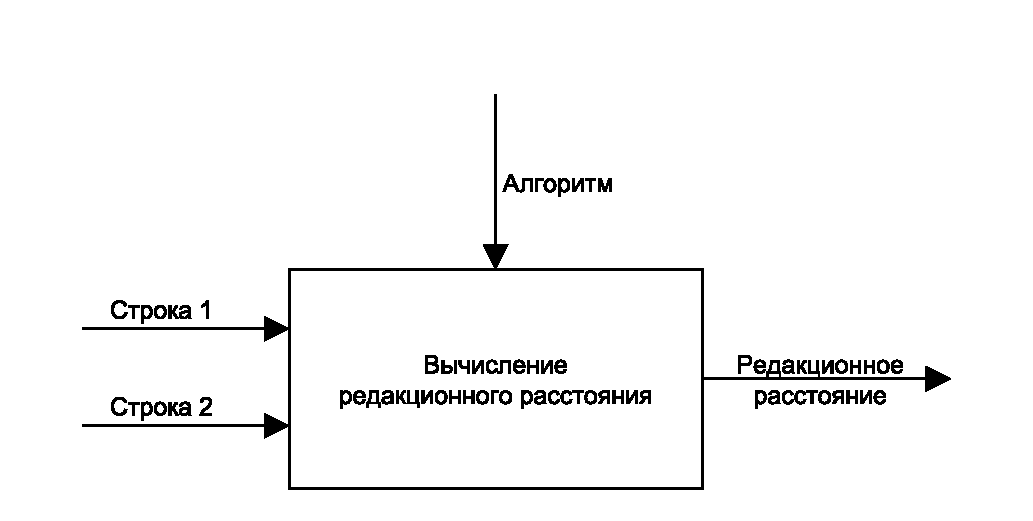
\includegraphics{pdf/mainIdef0.pdf}
    \caption{IDEF0 модель}
\end{figure}

\section{Разработка алгоритмов}
Для непосредственной реализации вышеописанных алгоритмов важно иметь их некоторые упрощённые визуальное представления, так как чтение таких представлений упрощает написание кода. Подходящим для этого вариантом визуализации являются схемы алгоритмов.

\subsection{Алгоритм Вагнера-Фишера}
Алгоритм Вагнера-Фишера является матричной реализацией поиска расстояния Левенштейна. Схема данного алгоритма приведена на рисунках 2.2 и 2.3.
\begin{figure}[H]
    \centering
    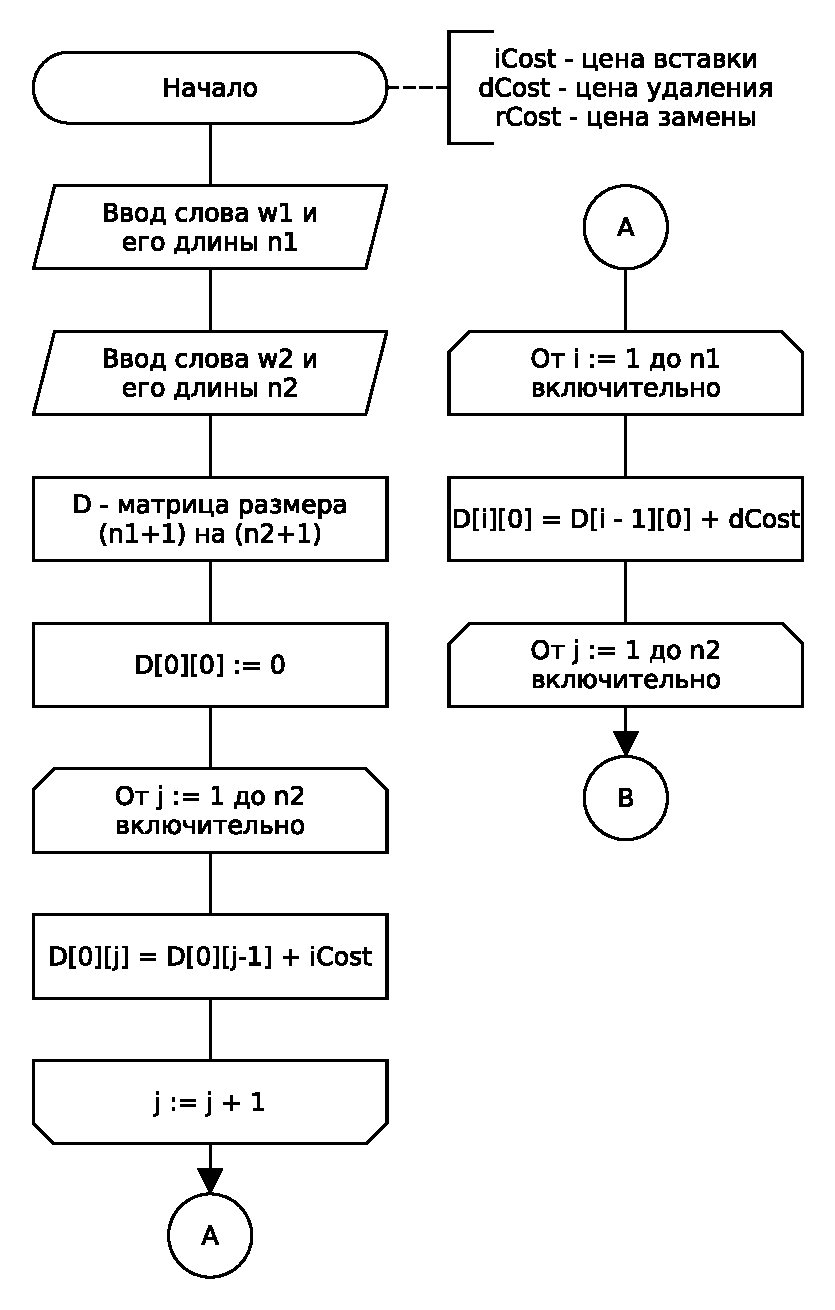
\includegraphics[scale=0.75]{pdf/wagner-fischer-part1.pdf}
    \caption{Алгоритм Вагнера-Фишера, часть 1}
\end{figure}
\begin{figure}[H]
    \centering
    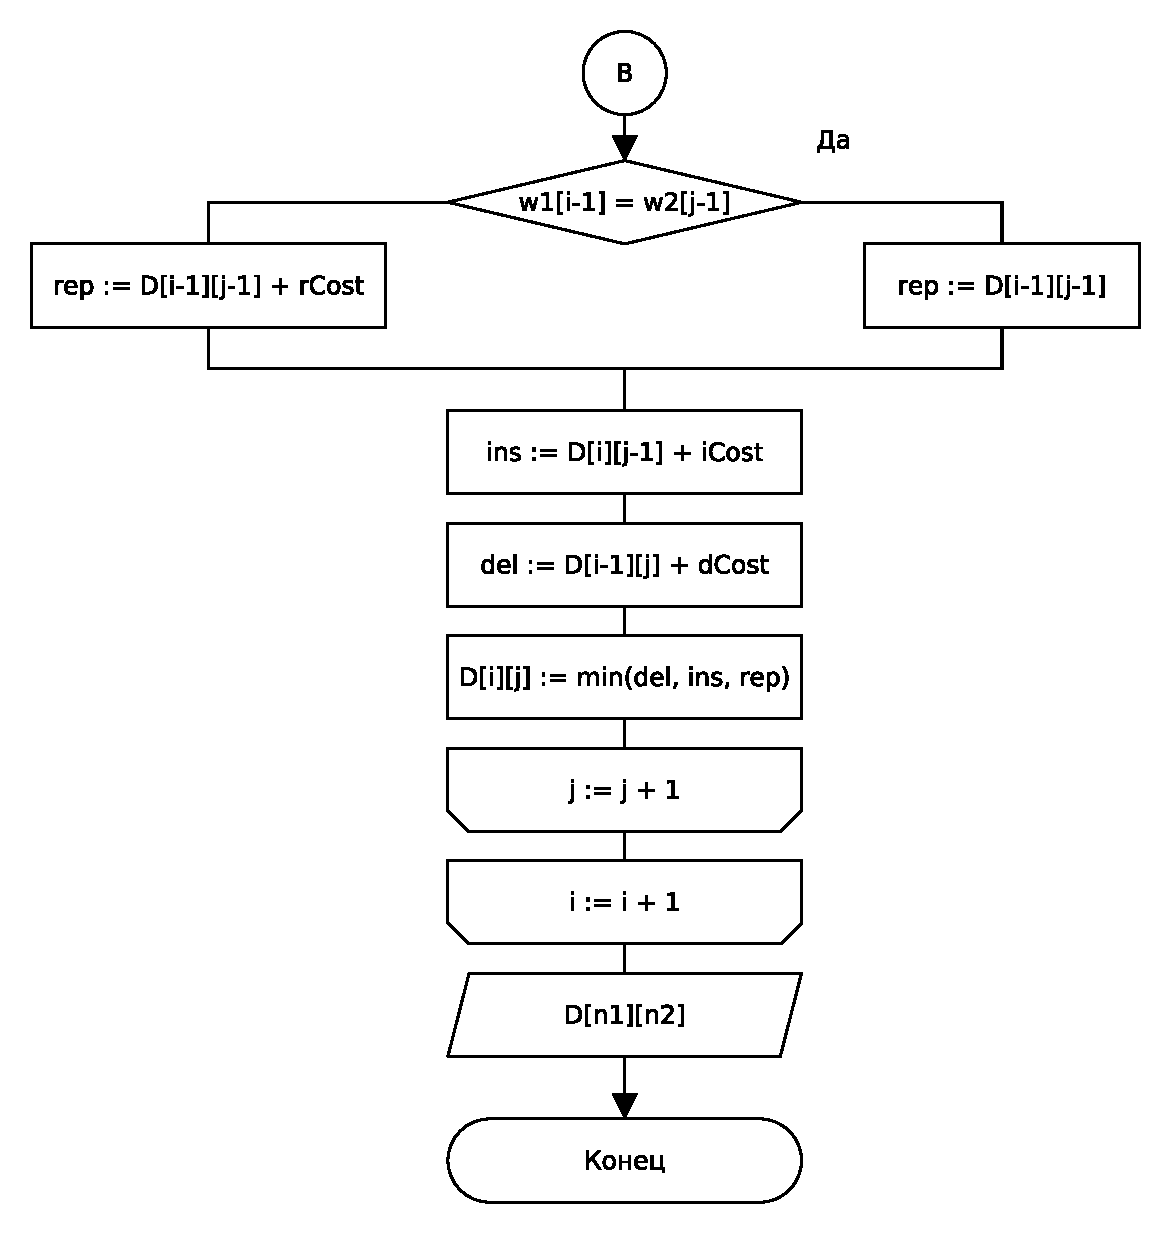
\includegraphics[scale=0.75]{pdf/wagner-fischer-part2.pdf}
    \caption{Алгоритм Вагнера-Фишера, часть 2}
\end{figure}

\subsection{Матричный алгоритм Дамерау-Левенштейна}
Матричный алгоритм Дамерау-Левенштейна представляет из себя модификацию алгоритма Вагнера-Фишера, в котором происходит дополнительная проверка на возможность проведения операции транспозиции. Схема данного алгоритма приведена на рисунках 2.4 и 2.5
\begin{figure}[H]
    \centering
    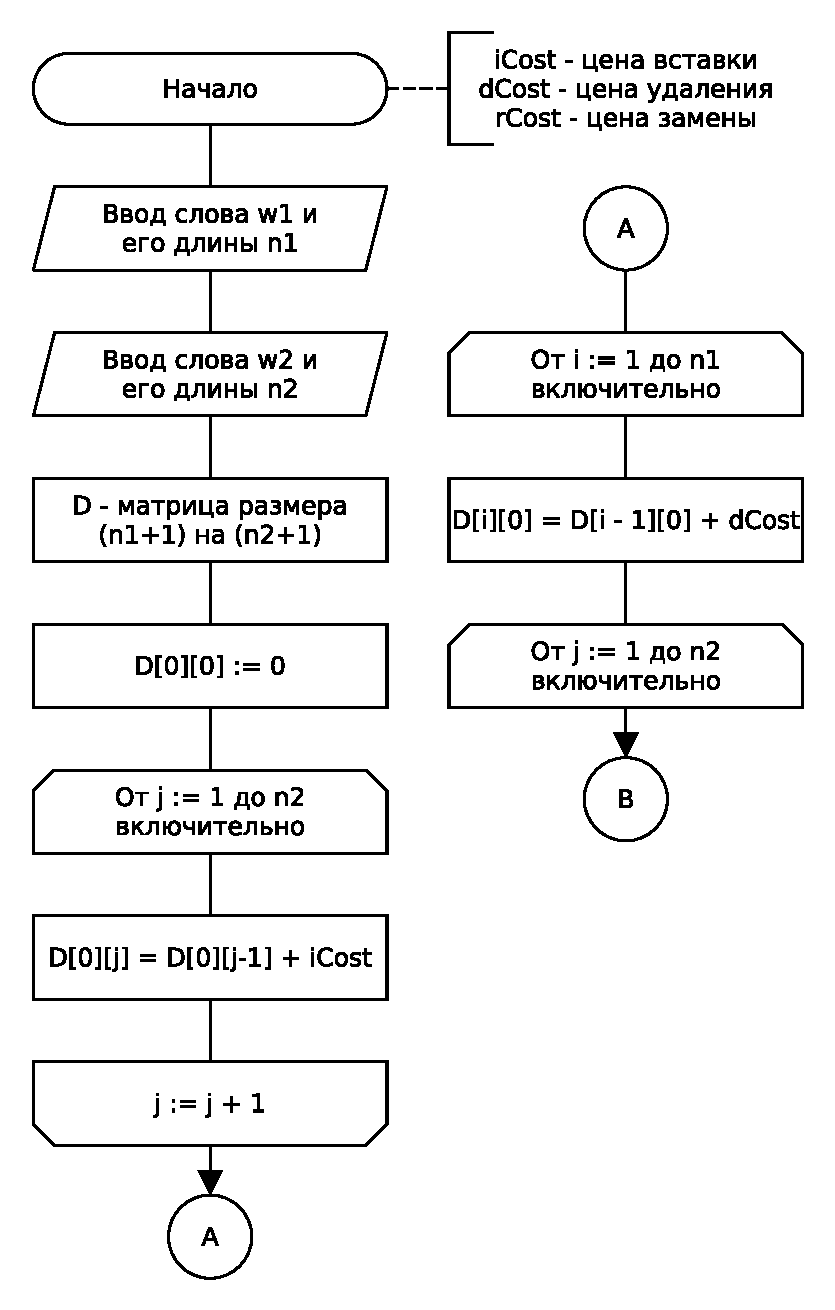
\includegraphics[scale=0.75]{pdf/damerau-levenshteain-part1.pdf}
    \caption{Матричный алгоритм Дамерау-Левенштейна, часть 1}
\end{figure}
\begin{figure}[H]
    \centering
    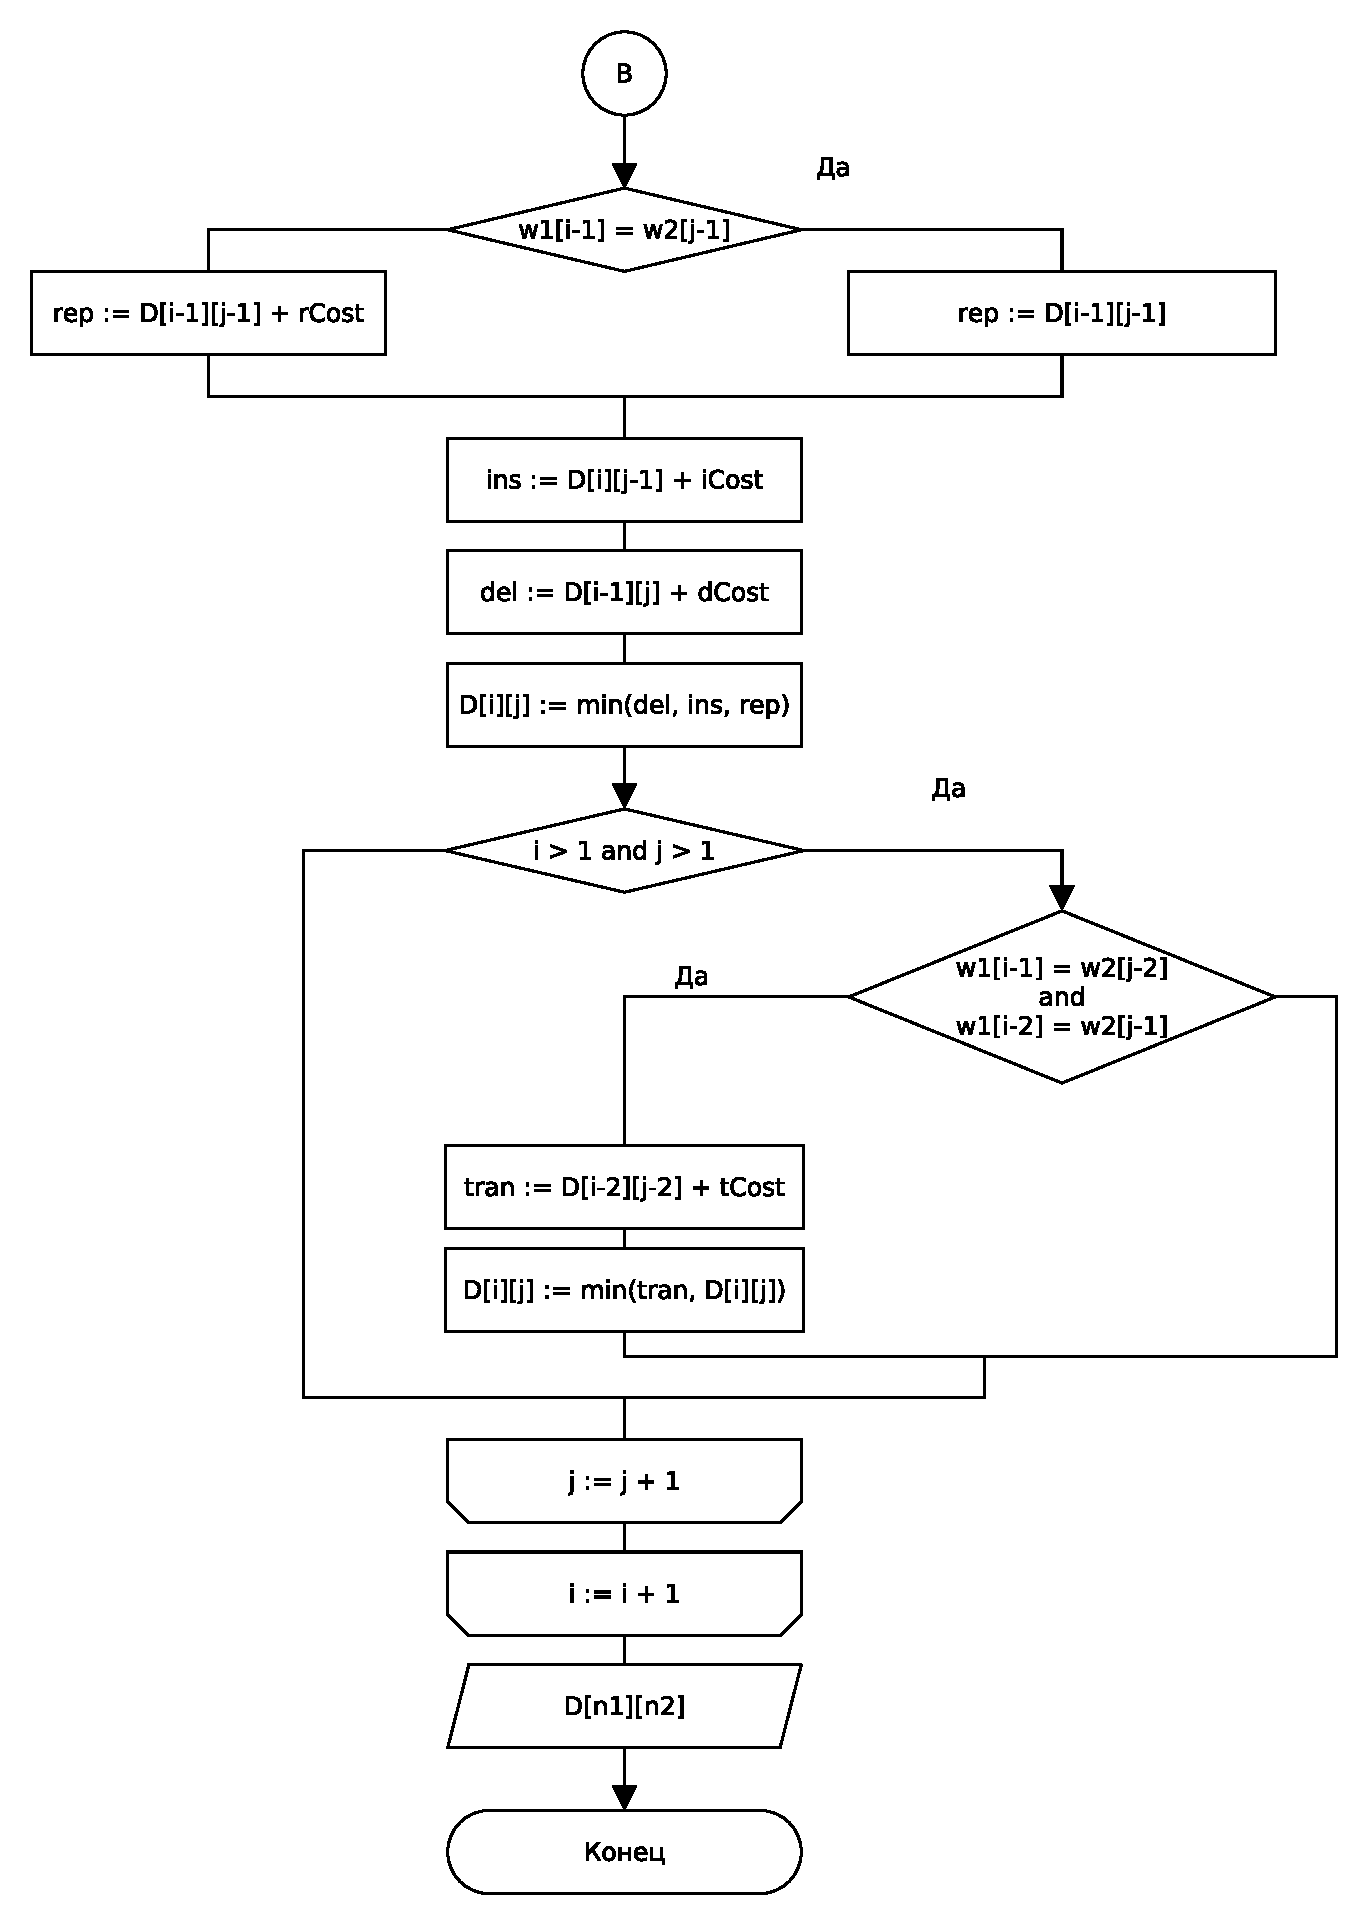
\includegraphics[scale=0.75]{pdf/damerau-levenshteain-part2.pdf}
    \caption{Матричный алгоритм Дамерау-Левенштейна, часть 2}
\end{figure}

\subsection{Рекурсивный алгоритм Дамерау-Левенштейна}
Суть рекурсивного алгоритма Левенштейна состоит в сведении поиска редакционного расстояния до тривиального случая, когда длина хотя бы одного из слов равна 0. Отличие алгоритма Левенштейна от алгоритма Дамерау-Левенштейна было описано ранее. Схема данного алгоритма приведена на рисунках 2.6, 2.7 и 2.8.
\begin{figure}[H]
    \centering
    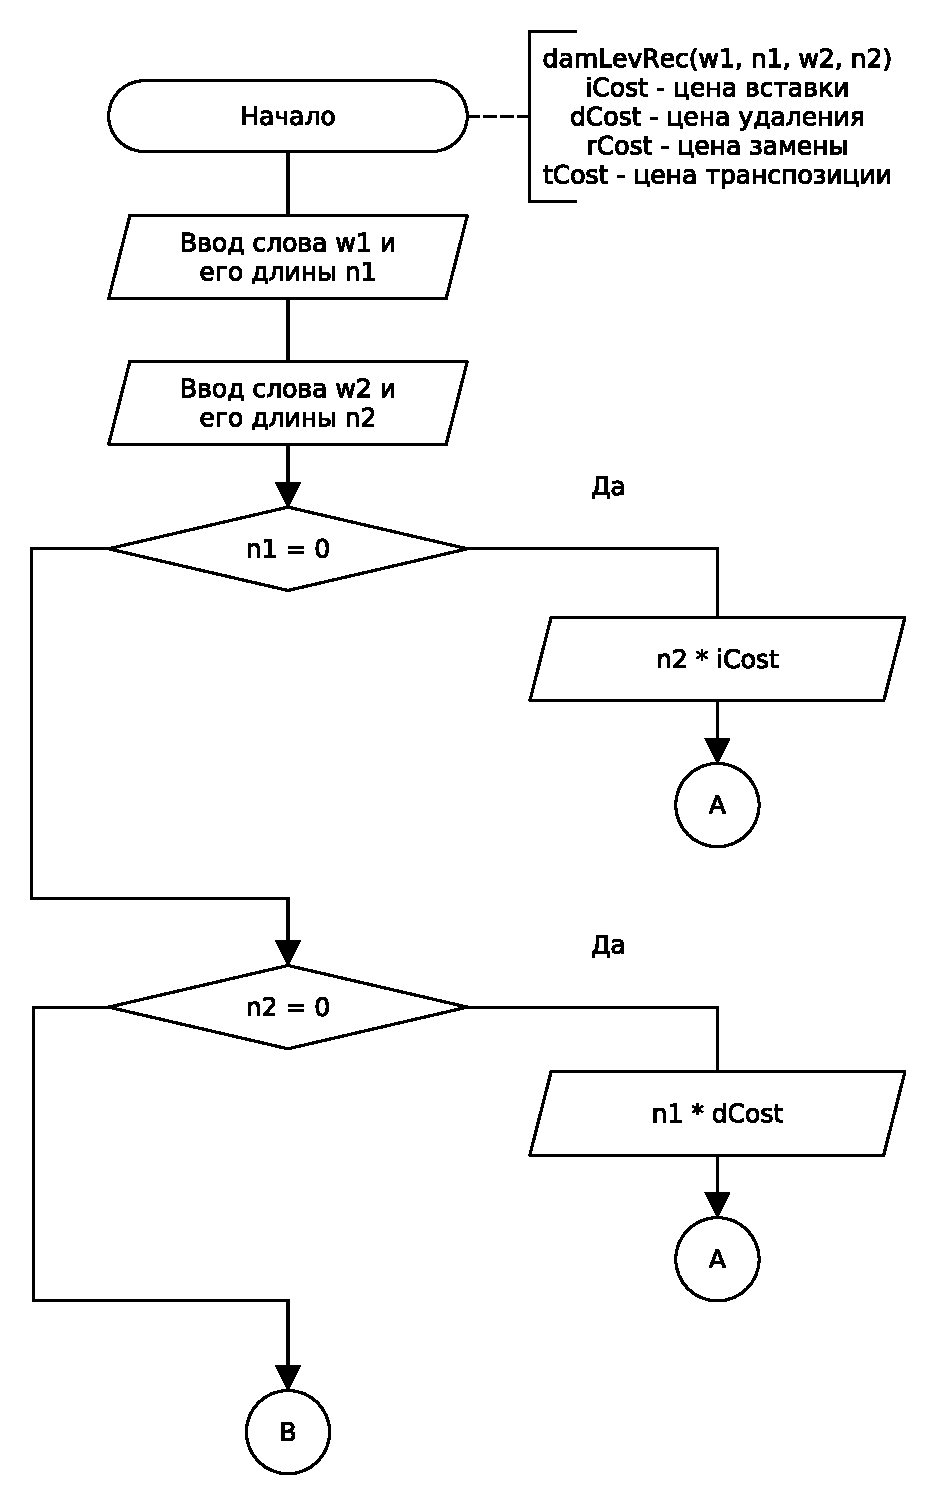
\includegraphics[scale=0.75]{pdf/damerau-levenshteainrec-part1.pdf}
    \caption{Рекурсивный алгоритм Дамерау-Левенштейна, часть 1}
\end{figure}
\begin{figure}[H]
    \centering
    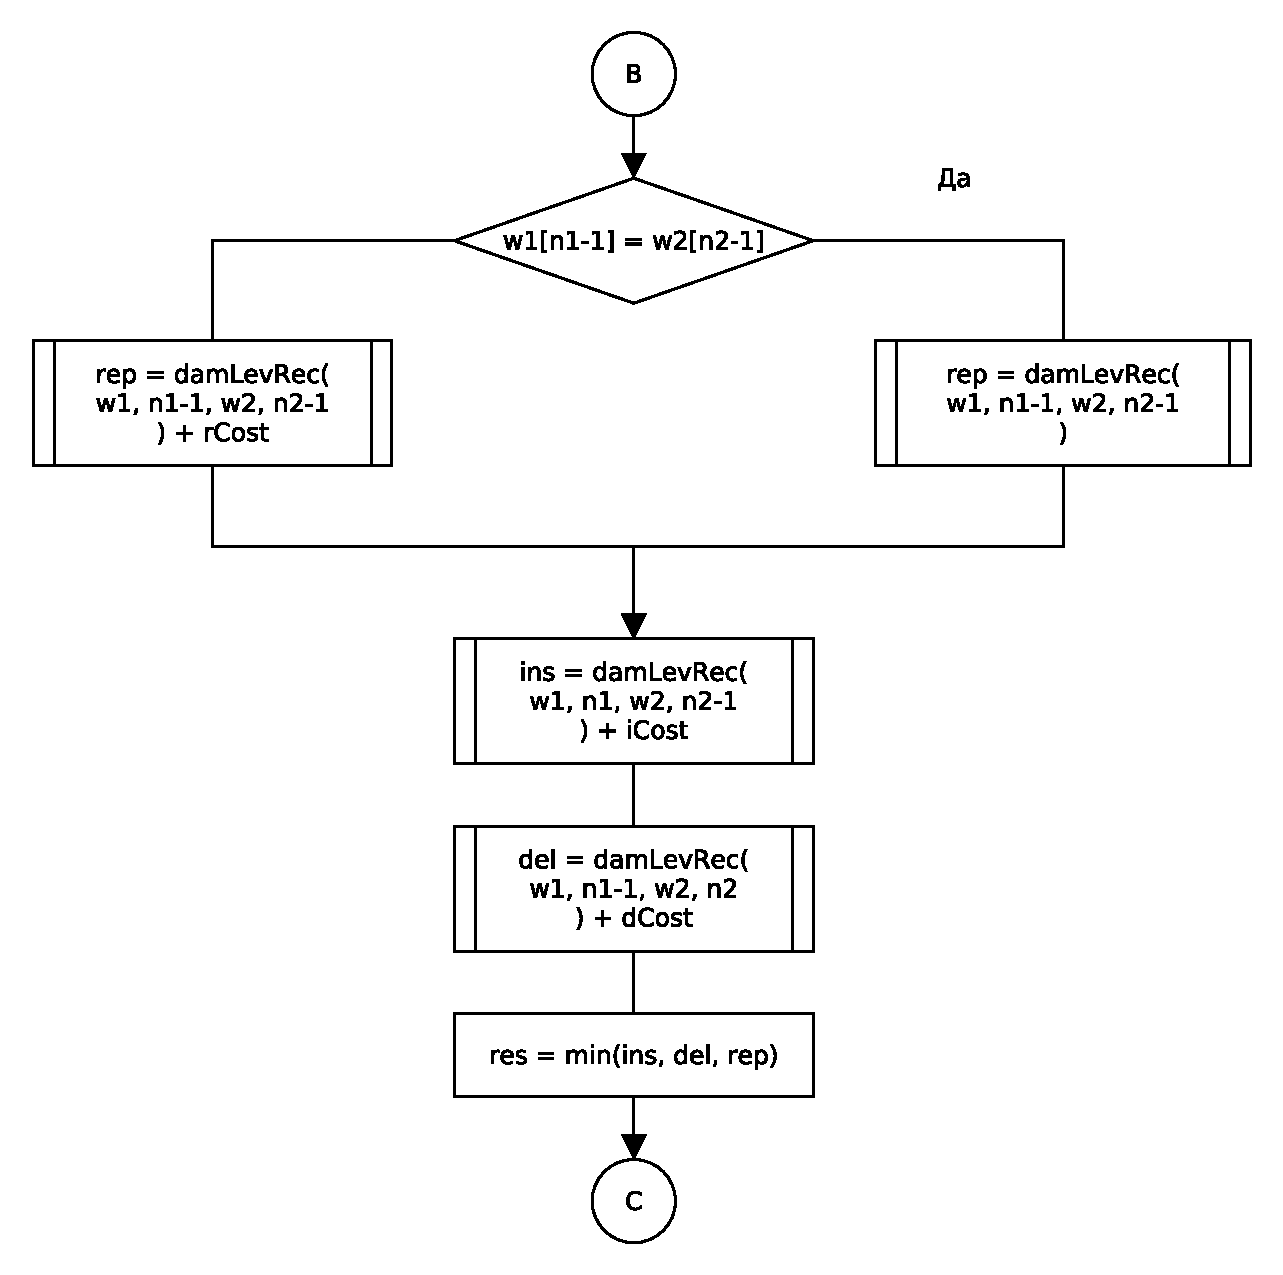
\includegraphics[scale=0.75]{pdf/damerau-levenshteainrec-part2.pdf}
    \caption{Рекурсивный алгоритм Дамерау-Левенштейна, часть 2}
\end{figure}
\begin{figure}[H]
    \centering
    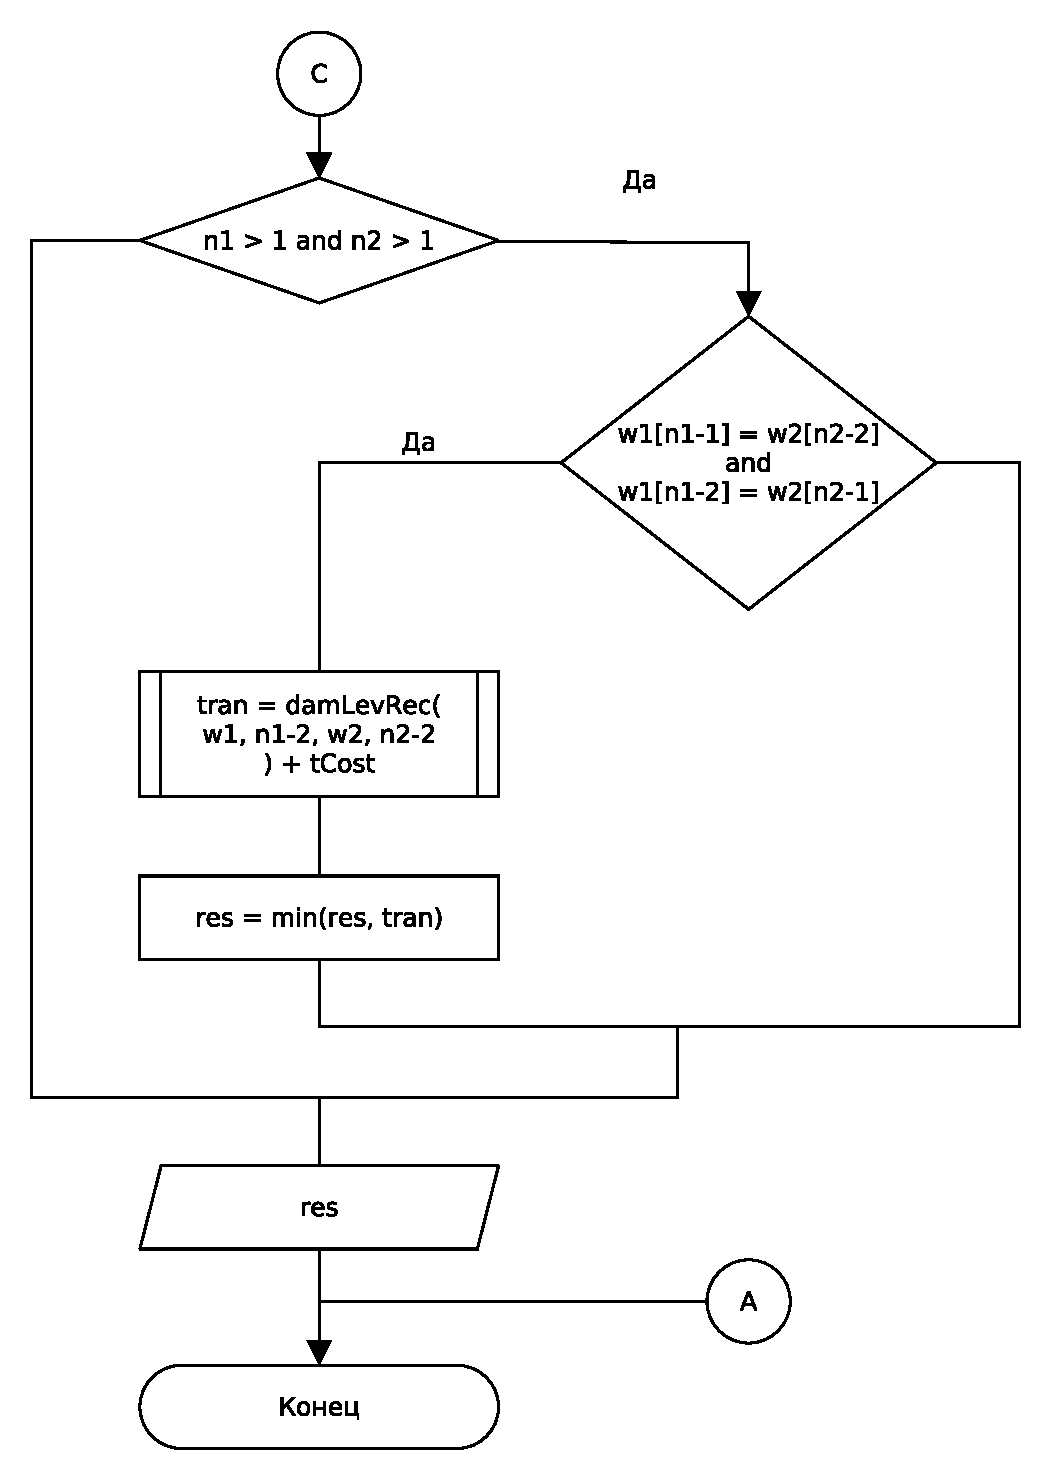
\includegraphics[scale=0.75]{pdf/damerau-levenshteainrec-part3.pdf}
    \caption{Рекурсивный алгоритм Дамерау-Левенштейна, часть 3}
\end{figure}

\section{Сравнительный анализ реализаций}
Для поиска редакционного расстояния можно применять как рекурсивные алгоритмы, так и матричные. Чтобы сделать вывод об эффективности того или иного алгоритма, проведём их анализ. Для упрощения задачи рассмотрим только алгоритмы поиска расстояния Левенштейна, так как объём затрачиваемых ресурсов этими алгоритмами прямо коррелирует с объёмом ресурсов, затрачиваемых алгоритмами поиска расстояния Дамерау-Левенштейна.

\subsection{Оценка сложности}
Произведем оценку общей сложности рекурсивного алгоритма. В рассмотренной реализации присутствуют 3 точки входа в рекурсию, условием выхода из рекурсии является равенство длины хотя бы одной из строк нулю. Из этого можно сделать вывод, что рекурсивный алгоритм Левенштейна в худшем случае имеет общую сложность \(O(3^n)\), где \(n\) - максимальная длина обрабатываемых слов.

Что касается матричной реализации, её задача сводится к полному обходу матрицы размера \((n_1+1)\cdot{}(n_2+1)\), где \(n_1\) и \(n_2\) - длины обрабатываемых строк. Следовательно, данный алгоритм имеет сложность \(O(n_1\cdot{}n_2)\).

\subsection{Оценка памяти}
Память, затрачиваемая на выполнение рассматриваемых алгоритмов зависит от используемых типов данных и соглашении о вызовах. В качестве примера, будем считать, что обрабатываемые строки передаются в функции по указателю, размер одного символа составляет 1 байт, целочисленного типа - 4 байта, указателя - 8 байт, используется cdecl (параметры функции передаются через стек, в который так же помещаются значения адреса возврата и указателя на верхушку текущего стекового кадра).

Как было показано ранее, в рекурсивной реализации происходит \(3^n + 3^{n-1} + ... + 3^0\) вызовов функции в худшем случае. Кроме того, важно то, что схема вызовов рекурсивного алгоритма имеет древовидную структуру, в которой для того же худшего случая глубина дерева достигает \(log_3(3^n) = n\). При этом вызовы, находящиеся на одном уровне дерева, не могут обрабатываться одновременно, то есть для всех вызовов одного уровня необходимо столько памяти, сколько нужно одному такому вызову. Допустим, что в аргументах функции передаются два указателя на обрабатываемые строки и 2 целочисленные переменные, означающие длины этих строк. Без учета возможного использования локальных переменных, имеем следующие затраты памяти:
\begin{equation}
    n \cdot{} (8+8 + 8+4 + 8+4) = 40 \cdot n
\end{equation}

В случае матричного алгоритма Дамерау-Левенштейна будем считать, что функция использует матрицу размера \((n_1+1)\cdot{}(n_2+1)\), указатель на начало этой матрицы и два целочисленных счётчика для циклов. Тогда имеем следующие затраты памяти:
\begin{equation}
    \begin{split}
    & 40 + (n_1+1)\cdot{}(n_2+1)\cdot{}4 + 8 + 4 + 4 = \\
    & 56 + 4\cdot{}(n_1+1)\cdot{}(n_2+1)
    \end{split}
\end{equation}

\subsection{Итог}
Таким образом, можно сделать вывод о том, что матричная реализация алгоритма поиска расстояния Левенштейна работает гораздо быстрее, чем рекурсивная, но и потребляет памяти так же гораздо больше.

